\section{Experiments} \label{sec: experiments}


\subsection{Rate-Distortion Performance} \label{sec: rate-distortion Performance}



\begin{figure}[t]
	\centering
	\begin{subfigure}{.5\textwidth}
		\centering
%		\includegraphics[width=.95\textwidth]{figures/psnr_vs_bpp_kodak.pdf}
		\caption{}
		\label{fig: psnr-vs-bpp kodak}
	\end{subfigure}%
	\begin{subfigure}{.5\textwidth}
		\centering
%		\includegraphics[width=.95\textwidth]{figures/ssim_vs_bpp_kodak.pdf}
		\caption{}
		\label{fig: ssim-vs-bpp kodak}
	\end{subfigure}
	\caption{Rate-distortion performance on the Kodak dataset. In panels (a) and (b), the average PSNR and SSIM are plotted against bits per pixel (bpp), respectively.}
	\label{fig: compression performance on kodak}
\end{figure}

\begin{figure}[t]
	\centering
	\begin{subfigure}{.5\textwidth}
		\centering
%		\includegraphics[width=.95\textwidth]{figures/psnr_vs_bpp_clic.pdf}
		\caption{}
		\label{fig: psnr-vs-bpp clic}
	\end{subfigure}%
	\begin{subfigure}{.5\textwidth}
		\centering
%		\includegraphics[width=.95\textwidth]{figures/psnr_vs_bpp_clic.pdf}
		\caption{}
		\label{fig: ssim-vs-bpp clic}
	\end{subfigure}
	\caption{Rate-distortion performance on the CLIC dataset. In panels (a) and (b), the average PSNR and SSIM are plotted against bits per pixel (bpp), respectively.}
	\label{fig: compression performance on clic}
\end{figure}


\begin{figure}[t]
	\centering
	\begin{subfigure}{\textwidth}
		\centering
		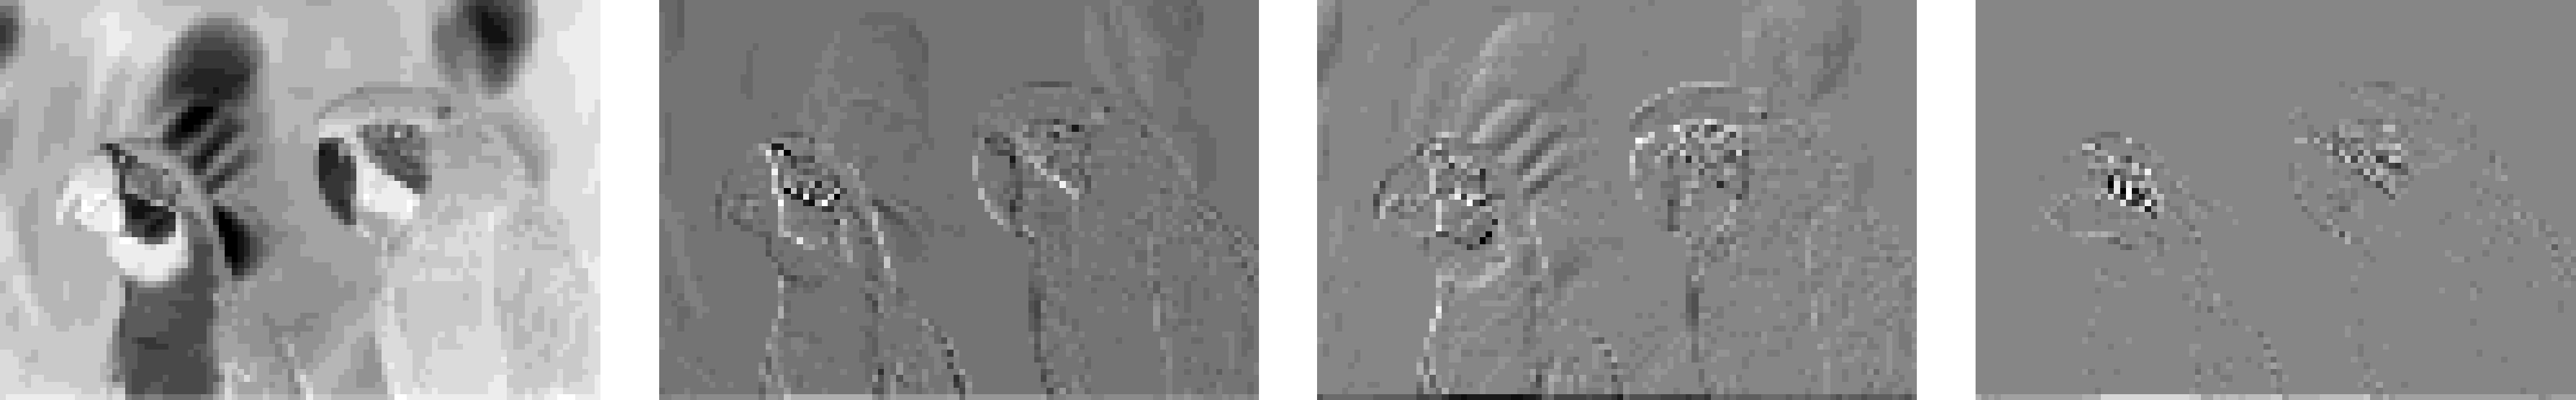
\includegraphics[width=.95\textwidth]{figures/kodim23_y_componets.pdf}
		\caption{}
		\label{fig: y componets}
	\end{subfigure}
	
	\begin{subfigure}{.455\textwidth}
		\centering
		\vspace{10pt}
		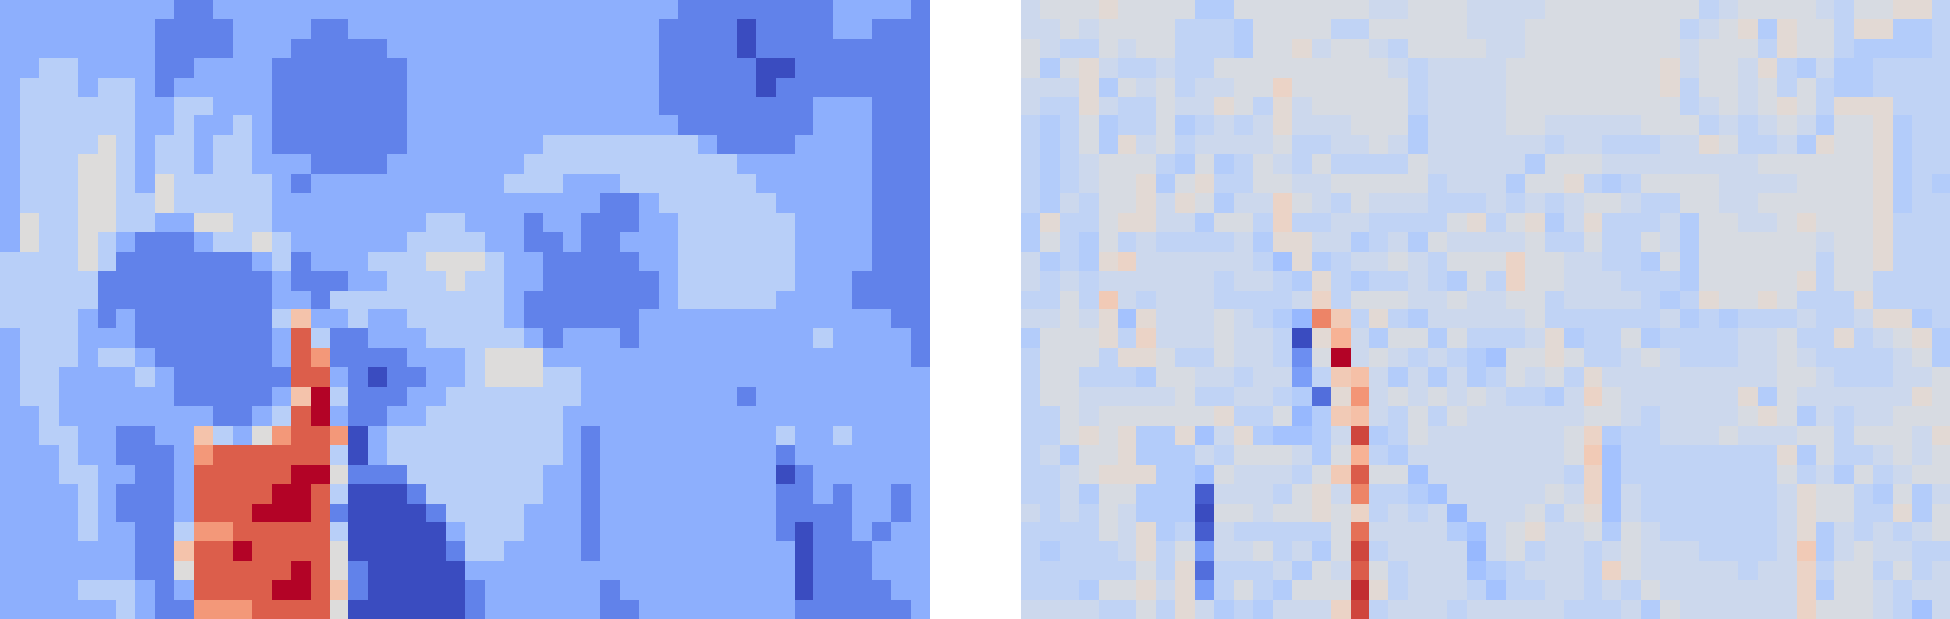
\includegraphics[width=.95\textwidth]{figures/kodim23_cb_componets.pdf}
		\caption{}
		\label{fig: cb componets}
	\end{subfigure}%
	\begin{subfigure}{.45\textwidth}
		\centering
		\vspace{10pt}
		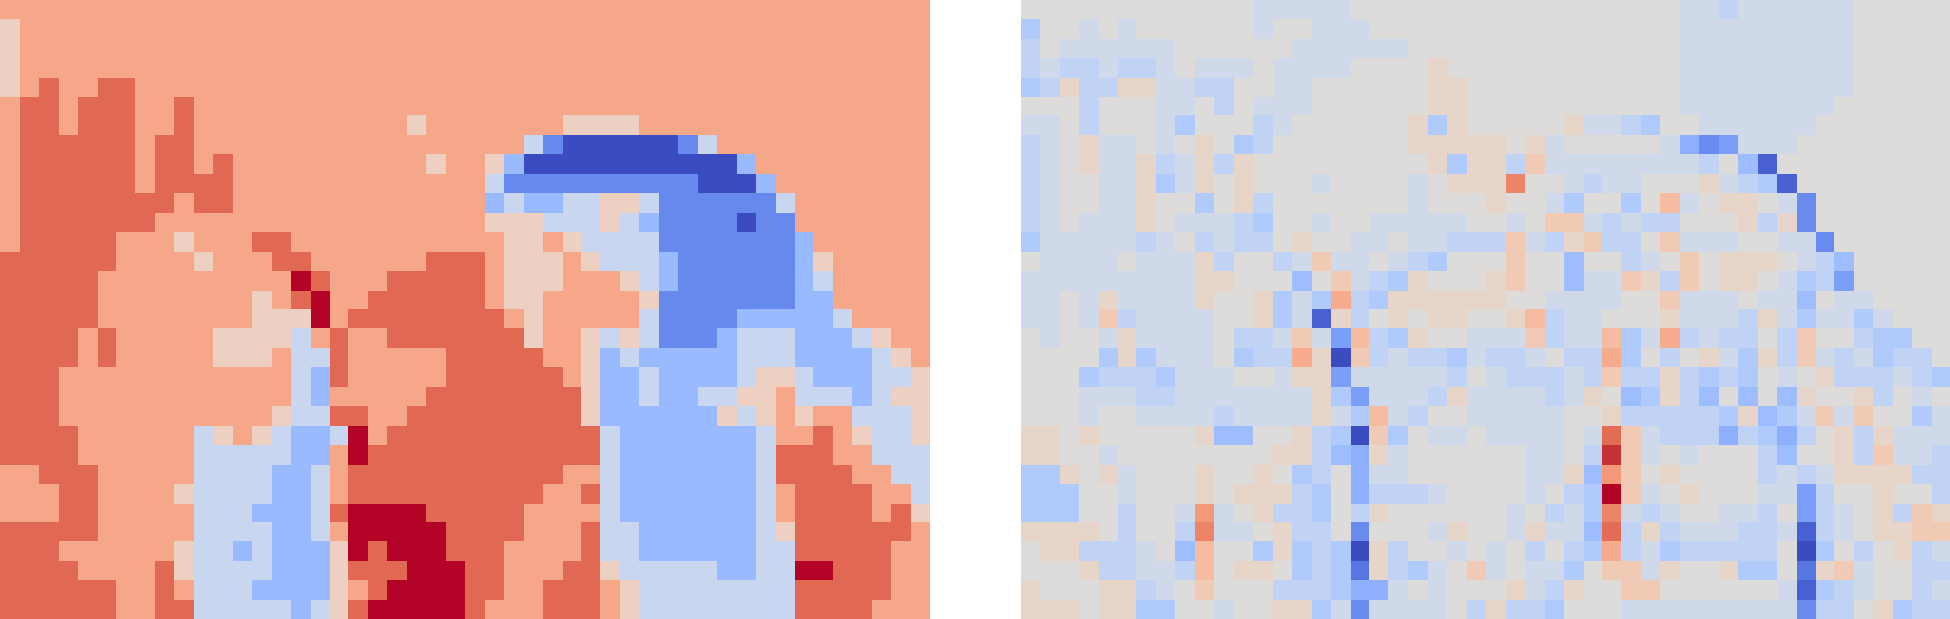
\includegraphics[width=.95\textwidth]{figures/kodim23_cr_componets.pdf}
		\caption{}
		\label{fig: cr componets}
	\end{subfigure}
	\caption{IMF components of the \texttt{kodim23} image from the Kodak dataset. Panels (a), (b), and (c) show the IMF components corresponding to luma (Y), blue-difference (Cb), and red-difference (Cr) chroma, respectively.}
	\label{fig: imf components}
\end{figure}



\subsection{ImageNet Classification Performance} \label{sec: imagenet Classification Performance}


\begin{figure}[t]
	\centering
	\begin{subfigure}{.5\textwidth}
		\centering
		%		\includegraphics[width=.95\textwidth]{figures/top1_vs_bpp_imagenet.pdf}
		\caption{}
		\label{fig: top1-vs-bpp imagenet}
	\end{subfigure}%
	\begin{subfigure}{.5\textwidth}
		\centering
		%		\includegraphics[width=.95\textwidth]{figures/top5_vs_bpp_imagenet.pdf}
		\caption{}
		\label{fig: top5-vs-bpp imagenet}
	\end{subfigure}
	\caption{Impact of different compression methods on ImageNet classification accuracy. Panels (a) and (b) show the validation top-1 and top-5 accuracy plotted against bits per pixel (bpp), respectively. A ResNet-50 model pretrained on the original ImageNet images was evaluated using validation images compressed by different methods.}
	
	\label{fig: compression impact on imagenet classification}
\end{figure}


\subsection{Ablation Studies} \label{sec: ablation studies}

\begin{figure}[t]
	\centering
	\begin{subfigure}{.5\textwidth}
		\centering
		%\includegraphics[width=.95\textwidth]{figures/patch_ablation_psnr_vs_bpp.pdf}
		\caption{}
		\label{fig: patch ablation psnr-vs-bpp}
	\end{subfigure}%
	\begin{subfigure}{.5\textwidth}
		\centering
		%\includegraphics[width=.95\textwidth]{figures/bounds_ablation_psnr_vs_bpp.pdf}
		\caption{}
		\label{fig: bounds ablation psnr-vs-bpp}
	\end{subfigure}
	
	\begin{subfigure}{.5\textwidth}
		\centering
		%\includegraphics[width=.95\textwidth]{figures/iteration_ablation_psnr_vs_bpp.pdf}
		\caption{}
		\label{fig: iteration ablation psnr-vs-bpp}
	\end{subfigure}%
	\begin{subfigure}{.5\textwidth}
		\centering
		%\includegraphics[width=.95\textwidth]{figures/colorspace_ablation_psnr_vs_bpp.pdf}
		\caption{}
		\label{fig: colorspace ablation psnr-vs-bpp}
	\end{subfigure}
	\caption{Ablation experiments for the IMF compression method. In all cases, we plot PSNR as a function of bits per pixel (bpp) on the Kodak dataset. (a) Compares IMF compression performance without patchification and different patch sizes. (b) Compares IMF compression performance for different bound values of factor matrices. (c) Compares IMF compression performance for different numbers of BCD iterations. (d) Compares IMF compression performance between RGB and YCbCr color space transform.}
	\label{fig: ablation studies}
\end{figure}

\paragraph{Patchification.} 

without patchification, patch size 4, 8, 16, 32

\paragraph{Factor bounds.} 

\paragraph{BCD iteration.}

\paragraph{Color space.}


